\documentclass{beamer}
\usetheme{Hannover}
\usepackage{fontspec, xunicode, xltxtra}
\XeTeXlinebreaklocale "zh"
\XeTeXlinebreakskip = 0.1pt plus 1pt minus 0.1pt
\usepackage{xeCJK} 
\usepackage{fontspec}  
\setCJKmainfont{SimSun} 
\setCJKmonofont{SimSun} 
\setmainfont{Courier}%{Times New Roman} {SourceCodePro-Regular}{Consolas}{Courier}
\usepackage{hyperref}
\usepackage[utf8]{inputenc} % this is needed for german umlauts
\usepackage[english]{babel} % this is needed for german umlauts
\usepackage[T1]{fontenc}    % this is needed for correct output 
                            % of umlauts in pdf
\usepackage{pgf,pgfarrows,pgfnodes,pgfautomata,pgfheaps}
\usepackage{amsmath,amssymb}
\usepackage{graphicx}
\usepackage{multimedia}
\usepackage{listings}
\lstset{language=C++}
\lstset{breaklines}
\lstset{extendedchars=false}

\graphicspath{{Figure/}}
\begin{document}
\title{数据结构大作业报告}
\subtitle{红黑树}
\author{姚皓天\\(2013011515)}

\date{2014年12月}
\subject{数据结构}

\begin{frame} 
\titlepage 
\end{frame} 

\begin{frame}
\frametitle{基本原理}
\section{基本原理}
\subsection{概述}
\begin{block}{概述}
本程序是由 Microsoft Visual Studio 2012 创建,目标框架为 .NET Framework 4.5。
程序实现了红黑树数据结构的可视化,实现了对学生成绩信息的输入输出以及检索的功能。\par
此外,实现了Hash表,用于管理学生的姓名和学号数据。
\end{block}
\subsection{原理}
\begin{block}{原理}
首先实现了将学生封装为Student类,接着封装为Node类,并在基础上创建红黑树,RBTree类。接着创建了HashTable<T>模板,实现了Hash表的功能。最后,在.NET框架下,完成图形界面的部署。
\end{block}
\end{frame}

\begin{frame}
\subsection{界面}
\begin{block}{界面}
\begin{figure}[H]
\centering
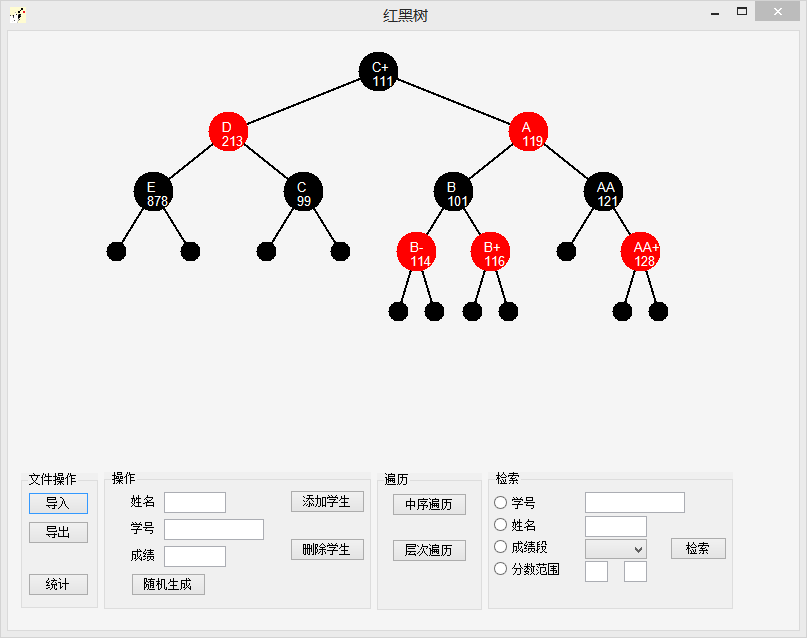
\includegraphics[width=0.8\textwidth]{2.png}
\caption{界面} 
\end{figure}
\end{block}
\end{frame}

\begin{frame}
\frametitle{操作说明}
\subsection{操作说明}
\begin{description}
\item[文件操作]
导入,导出按钮,可以从文本文件导入数据,或者导出到文本文件。统计信息按键可以显示实时的统计信息。
\item[添加删除]
输入学生的信息,就可以添加学生的信息,同时,上方的界面将同步绘制响应的红黑树可视化界面。输入学生的学号,就可以删除对应的学生。
\item[可视化]
点击节点,可以在弹出的对话框中查看节点的信息,同时在对话框中选中的条目信息可以回填到主界面中。
\item[遍历]
可以实现中序遍历和层次遍历两种方式的遍历。
\item[检索]
可以选择通过,姓名,学号,成绩段和分数区间四种不同的方式来检索学生成绩信息。
\end{description}
\end{frame}

\begin{frame}
\frametitle{程序设计}
\section{程序设计}
\begin{block}{概要设计}
\subsection{概要设计}
首先实现了将学生封装为Student类,接着封装为Node类,并在基础上创建红黑树,RBTree类。接着创建了HashTable<T>模板,实现了Hash表的功能。最后,在.NET框架下,完成图形界面的部署。
\end{block}
\begin{figure}[H]
\centering
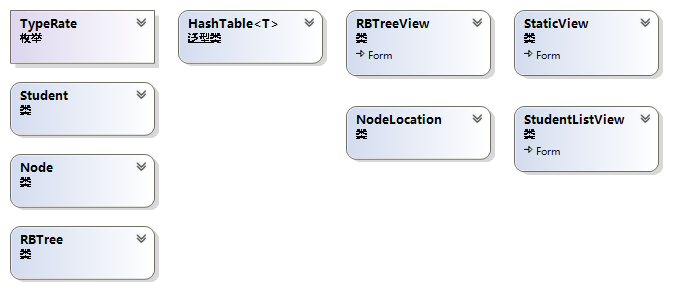
\includegraphics[width=0.8\textwidth]{1.png}
\caption{类图} 
\end{figure}
\end{frame}

\subsection{详细设计}
\begin{frame}
\frametitle{Student类}
\subsubsection{Student类}
\begin{figure}[H]
\centering
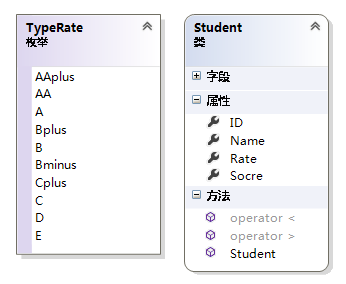
\includegraphics[scale = 0.4]{3.png}
\caption{Student类} 
\end{figure}
枚举型TypeRate描述成绩段。\par
Student类封装了学生的属性,并重载了operator< 和 opeartor > 通过分数段来实现对学生的比较,便于在红黑树中进行操作。
\end{frame}

\begin{frame}
\frametitle{RBTree类}
\subsubsection{RBTree类}
\begin{figure}[H]
\centering
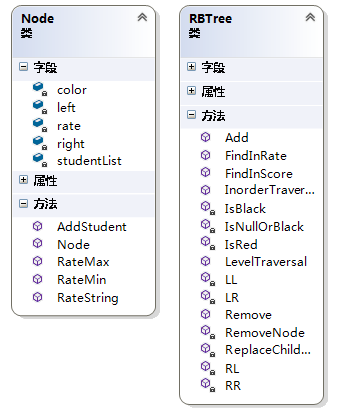
\includegraphics[scale = 0.4]{4.png}
\caption{红黑树的实现} 
\end{figure}
Node为红黑树中的每一个节点,包含的字段有颜色,关键码,左右子树,以及一个线性表用于保存数据。\par
RBTree实现了红黑树的插入,删除,查找,遍历等方法。其中树的旋转,换底作为私有方法,用于红黑树的维护。
\end{frame}

\begin{frame}
\subsubsection{HashTable类}
\begin{figure}[H]
\centering
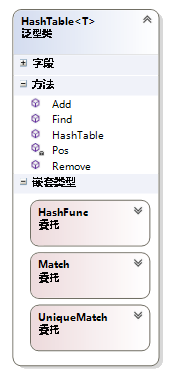
\includegraphics[scale = 0.4]{5.png}
\caption{HashTable的实现} 
\end{figure}
HashTable用泛型编写,实现添加,删除以及查找的功能。Hash函数的实现,查找匹配的方法使用委托编写,在实例化时实现。
\end{frame}

\begin{frame}
\frametitle{设计心得}
\section{设计心得}
\begin{block}{收获}
\subsection{收获}
这次大作业抛弃了年代久远的MFC框架,在全新的.NET Framework 4.5框架下完成了此处程序的编写。主要收获是熟悉了.NET Framework 以及编程语言C$\sharp$。
\end{block}
\begin{block}{特色}
\subsection{特色}
\begin{itemize}
\item 程序界面简洁。
\item 文本输入正则匹配:
\begin{figure}[H]
\centering
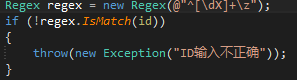
\includegraphics[scale = 0.8]{6.png}
\end{figure}
\end{itemize}
\end{block}
\end{frame}

\begin{frame}
\frametitle{版本库}
\url{https://github.com/yht1995/RBTree.git}
\begin{figure}[H]
\centering
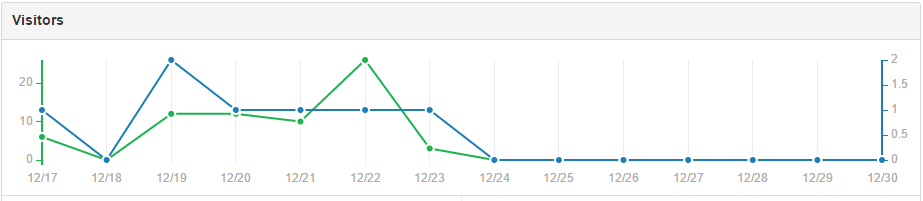
\includegraphics[scale = 0.4]{7.png}
\end{figure}
\end{frame}

\begin{frame}
\frametitle{附:红黑树高度的证明}
\section{附:红黑树高度的证明}
求证:包含n个内部节点的红黑树的高度是 O(log(n))。\par
定义:
h(v) = 以节点v为根的子树的高度。
bh(v) = 从v到子树中任何叶子的黑色节点的数目(如果v是黑色则不计数它)(也叫做黑色高度)。\par
\end{frame}
\begin{frame}
引理:以节点v为根的子树有至少$2^{bh(v) }− 1$个内部节点。\par
归纳基础:h(v) = 0时,bh(v) - 0,没有内部节点,$2^0-1=0$,结论成立。\par
归纳假设:若h(v) = k 的v有 $2^{bh(v)} − 1 $个内部节点,则 h(v') = k+1 的 v'有$2^{bh(v')}− 1 $个内部节点。\par
因为 v' 有 h(v') > 0 所以它是个内部节点。同样的它有黑色高度要么是 bh(v') 要么是 bh(v')-1 的两个儿子。它的内部节点数为
\[2^{bh(v') − 1} − 1 + 2^{bh(v') − 1} − 1 + 1 = 2^{bh(v')} − 1\]\par
结论证明:
因为在从根到叶子的任何路径上至少有一半的节点是黑色(根据红黑树属性4),根的黑色高度至少是h(root)/2。通过引理我们得到:
\[
n\geq 2^{\frac{h(root)}{2}}-1 \Leftrightarrow log(n+1) \geq \frac{h(root)}{2} \Leftrightarrow h(root)\leq 2log(n+1)
\]
\end{frame}
\end{document}